\section{Was ist Zeit?}

\begin{frame}{Was ist Zeit?}
    \begin{columns}
        \begin{column}{.65\textwidth}
            \textbf{Aristoteles} (300 BC.)
            \begin{quote}
                Die Zeit ist nichts Seiendes.
                Sie ist die \textbf{Wahrnehmung} des Davor und Danach an der \textbf{Bewegung}.
            \end{quote}
        \end{column}
        \begin{column}{.35\textwidth}
            \centering
            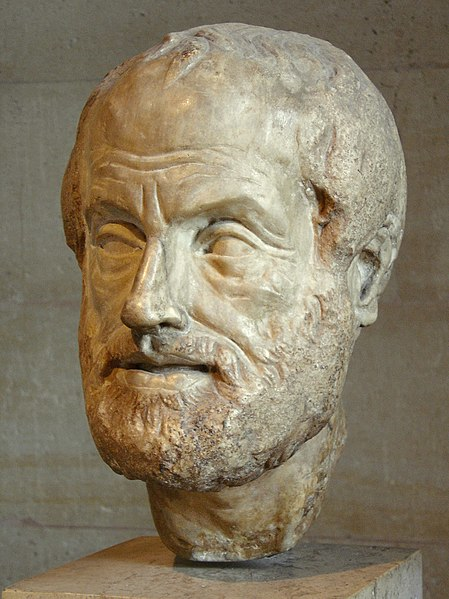
\includegraphics[height=.35\textheight]{img/aristoteles.png}\\
            \centering
            \scalebox{.4}{(After Lysippos [CC BY-SA 2.5])}
        \end{column}
    \end{columns}
    \begin{columns}
        \begin{column}{.35\textwidth}
            \centering
            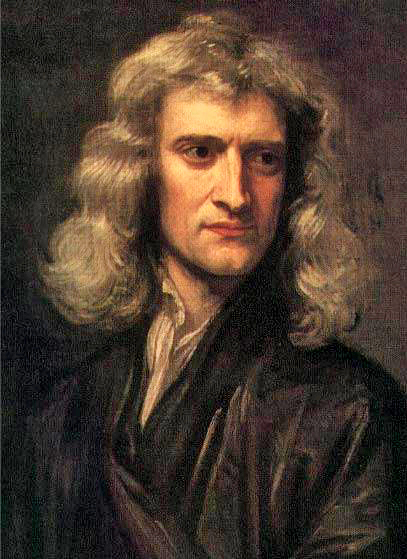
\includegraphics[height=.35\textheight]{img/newton.png}\\
            \centering
            \scalebox{.4}{(After Godfrey Kneller [Public domain])}
        \end{column}
        \begin{column}{.65\textwidth}
            \textbf{Newton} (1700 AD.)
            \begin{quote}
                Die absolute, wahre und mathematische Zeit fließt an sich und ihrer Natur nach gleichmäßig, \textbf{ohne Beziehung auf äußere Gegenstände}.
                (Insbesondere \textbf{unabhängig von einem Beobachter}.)
            \end{quote}
        \end{column}
    \end{columns}
\end{frame}

\begin{frame}{Was ist Zeit?}
    \begin{columns}
        \begin{column}{.55\textwidth}
            \textbf{2. Newtonsche Gesetz}
            \begin{quote}
            Um einen Körper (Masse $m$) zu beschleunigen ($v(t_1) \to v(t_2)$) braucht man Kraft $F$!
            \end{quote}

            \begin{equation*}
                F(t) \approx m \cdot \underbrace{\frac{v(t_2) - v(t_1)}{t_2 - t_1}}_{\text{Ableitung}}
            \end{equation*}
        \end{column}
        \begin{column}{.45\textwidth}
            \centering
            \includegraphics{img/taxis.png}\\
        \end{column}
    \end{columns}

    \centering
    In \textbf{Bewegungsgleichungen} verknüpfen Ableitungen Zeitpunkt $t$ mit \textbf{Vergangenheit} ($t_1$) und \textbf{Zukunft} ($t_2$)!
\end{frame}

\begin{frame}{Was ist Zeit?}
    \begin{columns}
        \begin{column}{.35\textwidth}
            \centering
            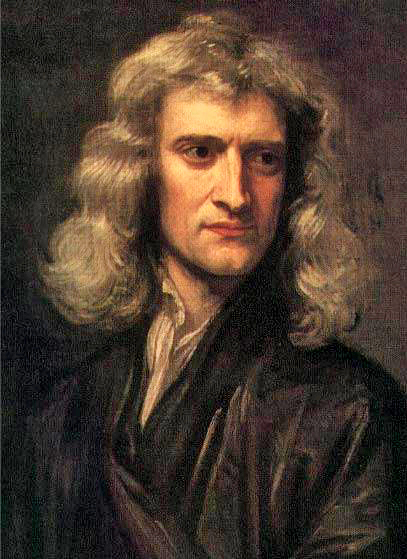
\includegraphics[height=.35\textheight]{img/newton.png}\\
            \centering
            \scalebox{.4}{(After Godfrey Kneller [Public domain])}
        \end{column}
        \begin{column}{.65\textwidth}
            \textbf{Newton}\\
            Physik beschreibt Natur im Raum (3D) und \textbf{unabhängig} davon in der absoluten Zeit.
        \end{column}
    \end{columns}
    \begin{columns}
        \begin{column}{.65\textwidth}
            \textbf{Einstein}\\
            Physik beschreibt Natur in \textbf{vier}dimensionaler Raumzeit.
            \begin{itemize}
                \item Zeit vergeht an verschiedenen Orten unterschiedlich schnell
            \end{itemize}
        \end{column}
        \begin{column}{.35\textwidth}
            \centering
            \includegraphics[height=.35\textheight]{img/einstein.png}\\
            \centering
            \scalebox{.4}{(Ferdinand Schmutzer [Public domain])}
        \end{column}
    \end{columns}
\end{frame}

\begin{frame}{Was ist Zeit?}
    \begin{columns}
        \begin{column}{.6\textwidth}
            \textbf{(Spezielle) Relativitätstheorie}\\
            \begin{itemize}
                \item In Bewegung vergeht die Zeit langsamer (Zwillingsparadoxon!)
                \item Gleichzeitigkeit ist subjektiv
                \item \textbf{Aber:} Kausalität bleibt stets gewahrt! (untere Grenzen für Zeitreisen)
            \end{itemize}
        \end{column}
        \begin{column}{.4\textwidth}
            \centering
            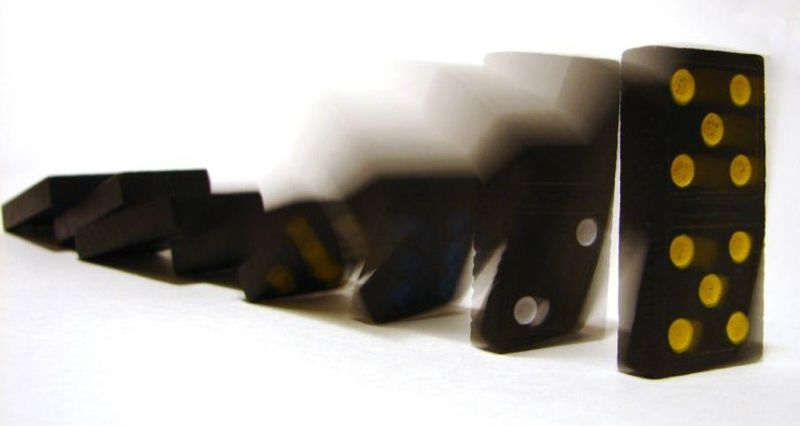
\includegraphics[height=.35\textheight]{img/cascade.png}\\
            \centering
            \scalebox{.4}{(aussiegall [CC BY 2.0])}
        \end{column}
    \end{columns}
\end{frame}

\begin{frame}{Was ist Zeit?}
    \begin{columns}
        \begin{column}{.65\textwidth}
            \textbf{Relativitätstheorie}\\
            \begin{itemize}
                \item Zeit vergeht an verschiedenen Orten unterschiedlich schnell
                \item Es gibt keine globale Gleichzeitigkeit
                \item Kausalität ist eine invariante und gilt in allen Bezugssystemen gleichermaßen
            \end{itemize}
        \end{column}
        \begin{column}{.35\textwidth}
            \centering
            \includegraphics[height=.35\textheight]{img/einstein.png}\\
            \centering
            \scalebox{.4}{(Ferdinand Schmutzer [Public domain])}
        \end{column}
    \end{columns}

    \begin{center}
        \scalebox{2.}{\&}
    \end{center}

    \textbf{Quantenphysik:} Materie und Raumzeit sind untrennbar (es gibt keinen leeren Raum!)
    \begin{center}
        $\Delta E \cdot \Delta t \ge \hbar / 2$
    \end{center}
\end{frame}
